\section{Szymon Kasperek}
\label{sec:skasperek}
% można tworzyć komentarze
\textbf{\textit{Wzór de Moivre'a}}

\begin{center}
    
\textbf{dla} \begin{math} z = |z|(cos\varphi + isin\varphi)\end{math}
\textbf{mamy}:

$z^n = |z|^ncos(n\varphi) + isin(n\varphi)$ $ \forall n\in N^+$
\\
\vspace{3mm}
Dodatkowe wyrażenie matematyczne, dodane w inny sposób:
\\
\vspace{1mm}
\begin{Large}\begin{math}E = mc^2 \end{math}\end{Large}
\end{center}
\vspace{1cm}
\centerline{\begin{Large}Zdjęcie kota mojego znajomego. (see Figure~\ref{fig:finek})\end{Large}}
\begin{figure}[htp]
    \centering
    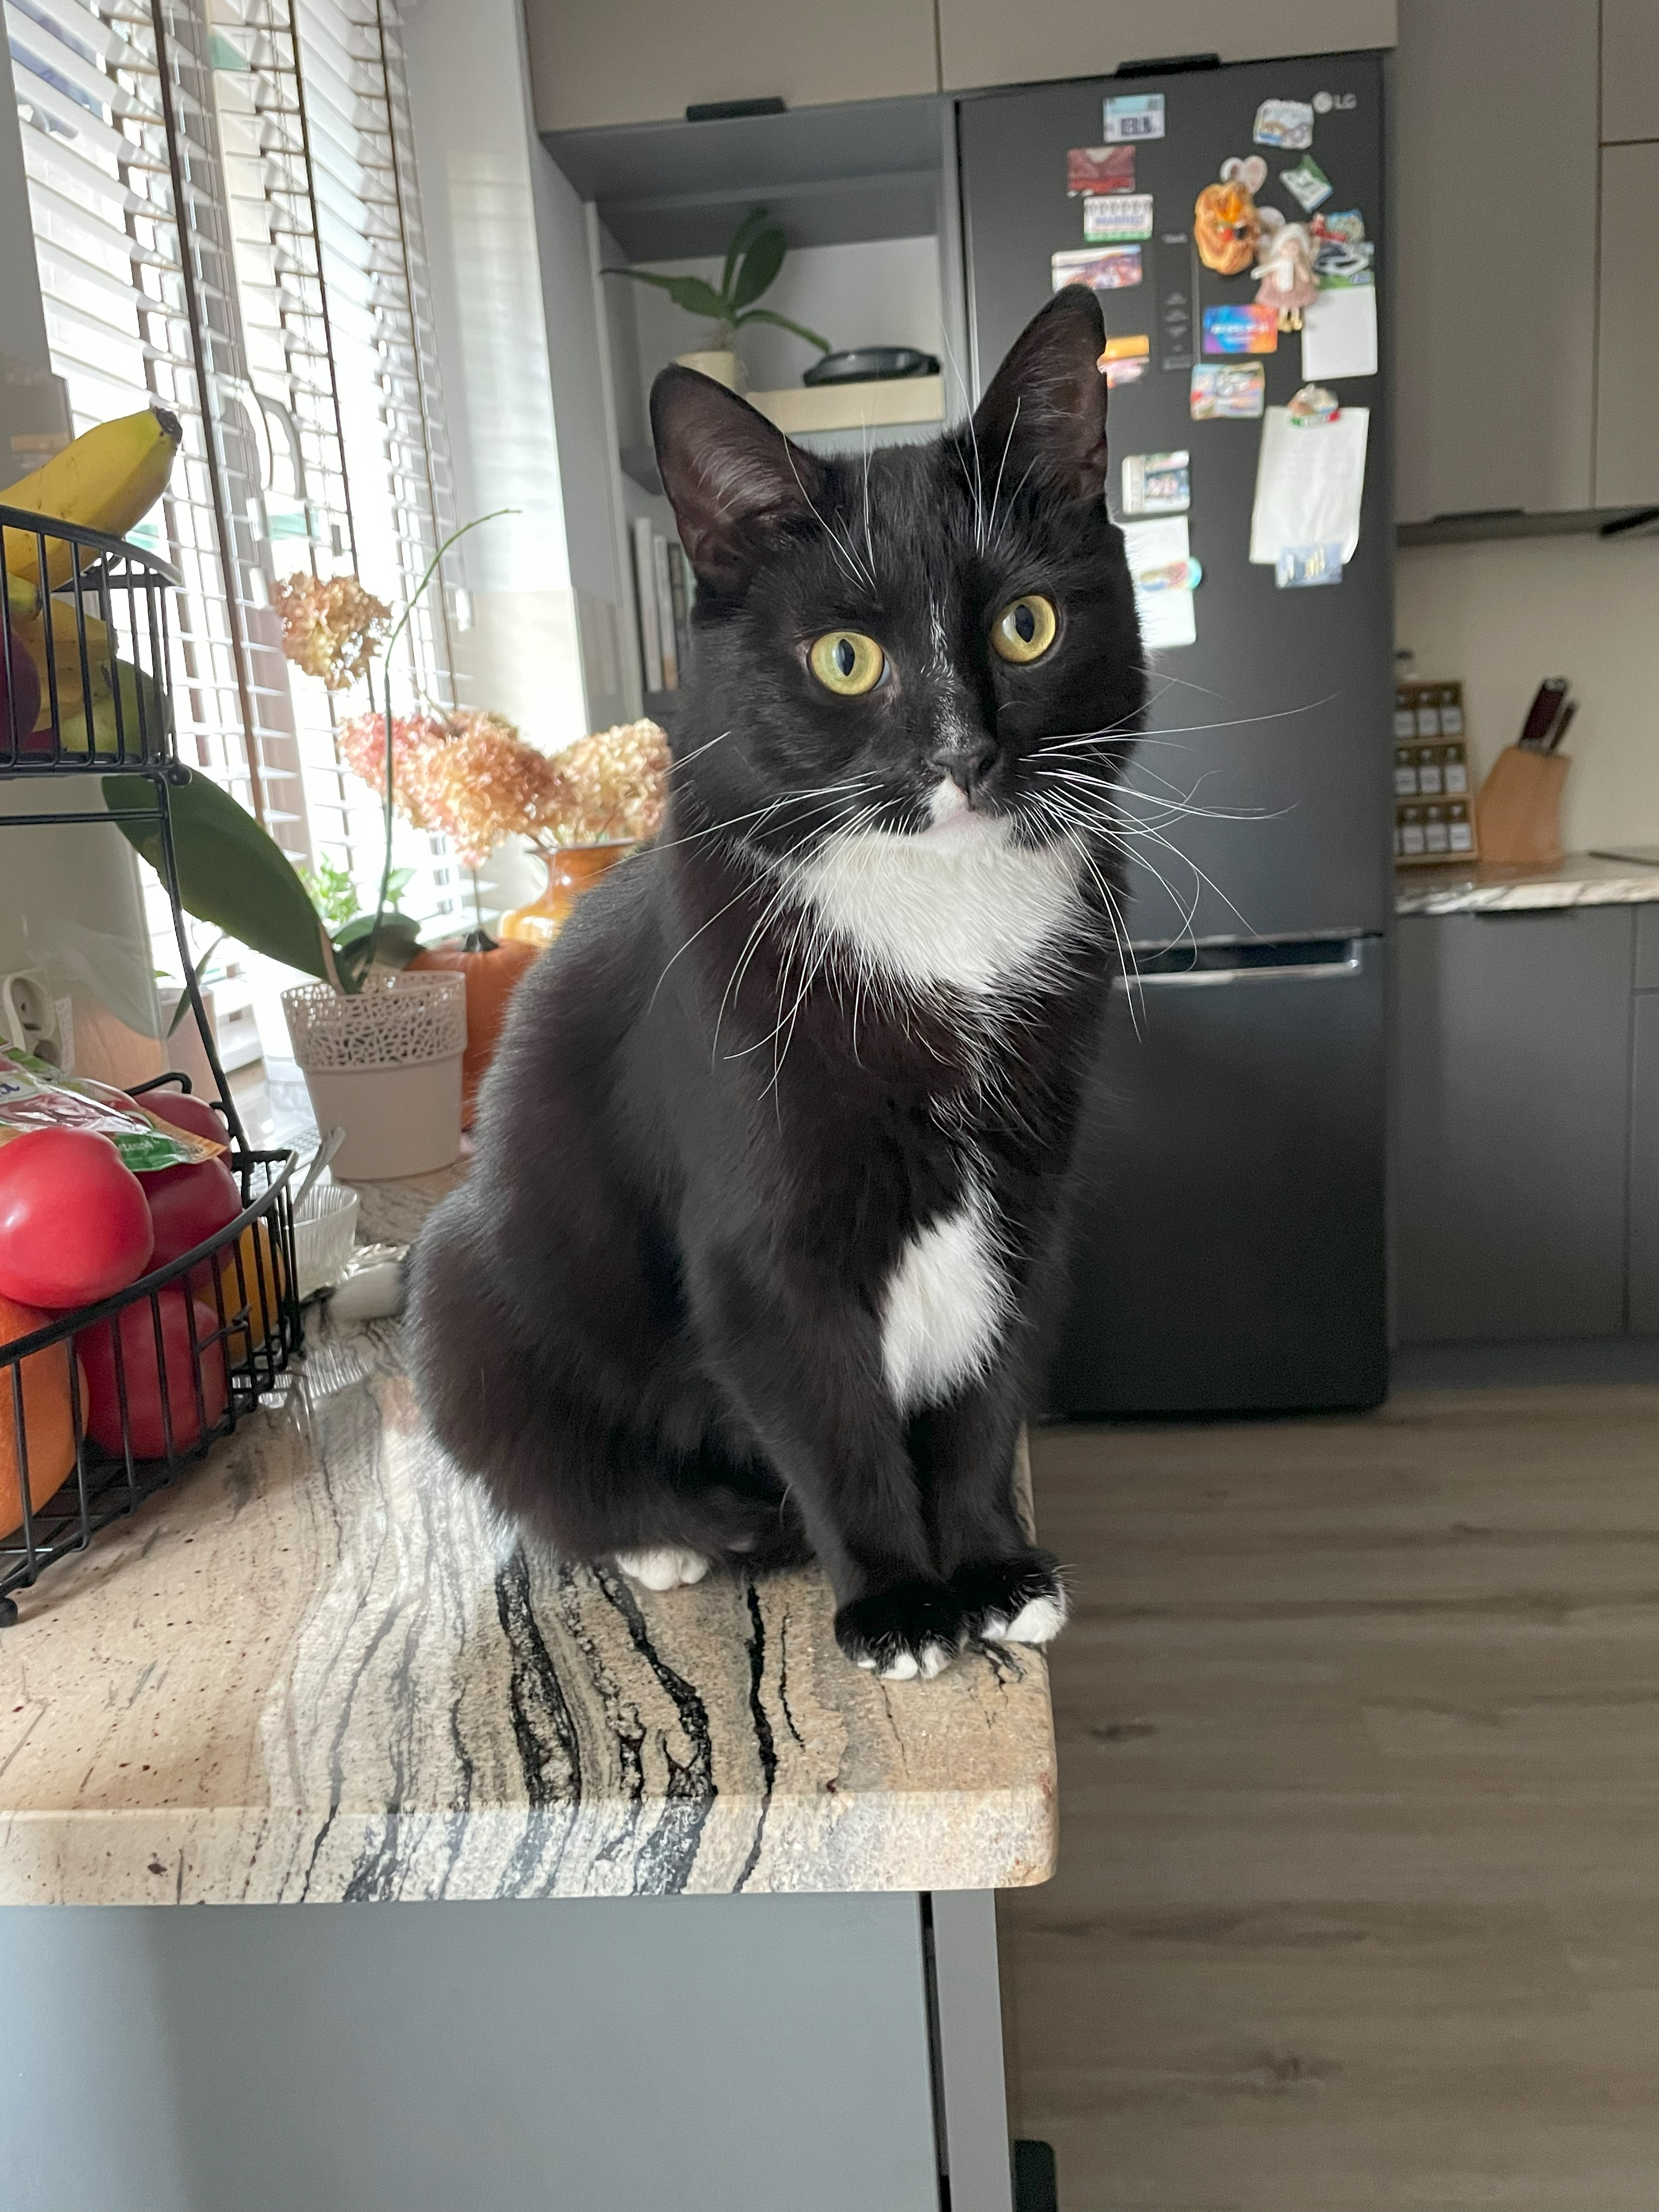
\includegraphics[width=0.6\linewidth]{pictures/finek.jpg}
    \caption{Kot \textbf{Finek}}
    \label{fig:finek}
\end{figure}
\centerline{Finek nie lubi głaskania i gryzie :(}
\newpage
Tabela~\ref{tab:table_SK} prezentuje połączenia znaków alfabetu od A do D.

\begin{table}[htbp]
\centering
\begin{tabular}{|c|c|c|c|c|}
\hline
  & A  & B  & C  & D  \\ \hline
A & AA & AB & AC & AD \\ \hline
B & BA & BB & BC & BD \\ \hline
C & CA & CB & CC & CD \\ \hline
D & DA & DB & DC & DD \\ \hline
\end{tabular}
\end{table}
\label{tab:table_SK}

W odniesieniu do Tabeli~\ref{tab:table_SK} poszczególne pola utworzone są w następujący sposób:
\begin{itemize}
    \item[$\circ$] AA - połączenie litery z \textbf{pierwszego rzędu} i \textbf{pierwszego wiersza} (A oraz A)
    \item[!] AB - połączenie litery z \textbf{pierwszego rzędu} i \textbf{drugiego wiersza} (A oraz B)
    \item[$\bullet$] CD - połączenie litery z \textbf{trzeciego rzędu} i \textbf{czwartego wiersza} (C oraz D)
    \item[$\rightarrow$] \begin{large}\textbf{itp.}\end{large}
\end{itemize}
Dodatkowo:
\begin{enumerate}
    \item Dane w rzędzie rozpoczynają się od \textbf{tej samej \textit{litery}}
    \item Dane w wierszu kończą się \texttt{tą samą literą}
\end{enumerate}
\vspace{1mm}

\centerline{\begin{Large} \textbf{Co autor rozdziału miał na myśli?} \end{Large}}
\begin{flushleft}
\setlength{\parindent}{20pt}
\par
Podane powyżej treści stanowią informacyjnie-edukacyjne \textbf{\underline{zero}}. Dane te są jedynie napisanym \begin{Large}\textit{bełkotem}\end{Large}, który pomaga nauczyć się konstruowania dokumentów w \begin{huge}\LaTeX\end{huge}. Nie stanowią żadnych wartościowych danych pomocnych w życiu, a jedynie powodują stratę czasu dla osoby, która zdecydowała się przeczytać poszczególne akapity
\par
Na zademonstrowanie braku wartości tekstu wklejam \emph{randomowy} ciąg z generatora \textbf{Lorem ipsum}: 
\par
\texttt{Lorem ipsum} dolor sit amet, \textbf{consectetur adipiscing} elit. Suspendisse lacinia purus id ipsum ultrices, quis finibus orci maximus. Vivamus sed libero non justo pulvinar maximus. Etiam interdum cursus lorem, \underline{\textit{nec vestibulum} erat euismod eu.} Proin aliquam nibh metus, non viverra sapien vestibulum id. Proin aliquam et mauris eget aliquam. 
\par
Przywołuję również kota mojego kolegi ze zdjęcia~\ref{fig:finek}, żeby pokazać użycie odwołań do zdjęcia, czy tabeli (np. tabela~\ref{tab:table_SK})
\end{flushleft}
\centerline{\begin{small} \textbf{Zmiana w pliku z Overleafa na githuba} \end{small}}